\begin{example} \label{eg:6.3.2} % EXAMPLE
Find the arc length of $\ds f(x) =\frac18x^2-\ln x$ from $x=1$ to $x=2$.

\solution
This function was chosen specifically because the resulting integral can be evaluated exactly. We begin by finding $\fp(x) = x/4-1/x$. The arc length is 
\begin{align*}
L		&=  \int_1^2 \sqrt{1+ \left(\frac x4-\frac1x\right)^2}\ dx \\
		&= 	\int_1^2 \sqrt{1 + \frac{x^2}{16} -\frac12 + \frac1{x^2} } \ dx \\
\end{align*}
\begin{align*}
\phantom{L}
		&=	\int_1^2 \sqrt{\frac{x^2}{16} +\frac12 + \frac1{x^2} } \ dx \\
		&=	\int_1^2	\sqrt{ \left(\frac x4 + \frac1x\right)^2}\ dx \\
		&= \int_1^2 \left(\frac x4 + \frac1x\right) \ dx \\
		&=  \left(\frac{x^2}8 + \ln x\right)\Bigg|_1^2\\
		&=	\frac38+\ln 2 \approx 1.07 \ \text{units}.
\end{align*}
	
A graph of $f$ is given in Figure \ref{F:6.3.Ex2}; the portion of the curve measured in this problem is in bold.

\end{example}

\begin{marginfigure}[-8cm] %MARGIN FIGURE
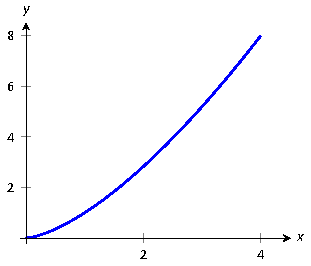
\includegraphics{figures/figarc1}
\caption{A graph of $f(x) = \frac18x^2-\ln x$ from Example~\ref{eg:6.3.2}.} \label{F:6.3.Ex2}
\end{marginfigure}

